% Options for packages loaded elsewhere
\PassOptionsToPackage{unicode}{hyperref}
\PassOptionsToPackage{hyphens}{url}
%
\documentclass[
  12pt,
  oneside]{book}
\usepackage{lmodern}
\usepackage{setspace}
\usepackage{amsmath}
\usepackage{ifxetex,ifluatex}
\ifnum 0\ifxetex 1\fi\ifluatex 1\fi=0 % if pdftex
  \usepackage[T1]{fontenc}
  \usepackage[utf8]{inputenc}
  \usepackage{textcomp} % provide euro and other symbols
  \usepackage{amssymb}
\else % if luatex or xetex
  \usepackage{unicode-math}
  \defaultfontfeatures{Scale=MatchLowercase}
  \defaultfontfeatures[\rmfamily]{Ligatures=TeX,Scale=1}
\fi
% Use upquote if available, for straight quotes in verbatim environments
\IfFileExists{upquote.sty}{\usepackage{upquote}}{}
\IfFileExists{microtype.sty}{% use microtype if available
  \usepackage[]{microtype}
  \UseMicrotypeSet[protrusion]{basicmath} % disable protrusion for tt fonts
}{}
\makeatletter
\@ifundefined{KOMAClassName}{% if non-KOMA class
  \IfFileExists{parskip.sty}{%
    \usepackage{parskip}
  }{% else
    \setlength{\parindent}{0pt}
    \setlength{\parskip}{6pt plus 2pt minus 1pt}}
}{% if KOMA class
  \KOMAoptions{parskip=half}}
\makeatother
\usepackage{xcolor}
\IfFileExists{xurl.sty}{\usepackage{xurl}}{} % add URL line breaks if available
\IfFileExists{bookmark.sty}{\usepackage{bookmark}}{\usepackage{hyperref}}
\hypersetup{
  pdftitle={Spatial pattern mining of tech clusters of dynamics and industry mix based on quantitative methods in England area, UK},
  hidelinks,
  pdfcreator={LaTeX via pandoc}}
\urlstyle{same} % disable monospaced font for URLs
\usepackage[left=4cm, right=3cm, top=2.5cm, bottom=2.5cm]{geometry}
\usepackage{longtable,booktabs}
% Correct order of tables after \paragraph or \subparagraph
\usepackage{etoolbox}
\makeatletter
\patchcmd\longtable{\par}{\if@noskipsec\mbox{}\fi\par}{}{}
\makeatother
% Allow footnotes in longtable head/foot
\IfFileExists{footnotehyper.sty}{\usepackage{footnotehyper}}{\usepackage{footnote}}
\makesavenoteenv{longtable}
\usepackage{graphicx}
\makeatletter
\def\maxwidth{\ifdim\Gin@nat@width>\linewidth\linewidth\else\Gin@nat@width\fi}
\def\maxheight{\ifdim\Gin@nat@height>\textheight\textheight\else\Gin@nat@height\fi}
\makeatother
% Scale images if necessary, so that they will not overflow the page
% margins by default, and it is still possible to overwrite the defaults
% using explicit options in \includegraphics[width, height, ...]{}
\setkeys{Gin}{width=\maxwidth,height=\maxheight,keepaspectratio}
% Set default figure placement to htbp
\makeatletter
\def\fps@figure{htbp}
\makeatother
\setlength{\emergencystretch}{3em} % prevent overfull lines
\providecommand{\tightlist}{%
  \setlength{\itemsep}{0pt}\setlength{\parskip}{0pt}}
\setcounter{secnumdepth}{5}
\usepackage[none]{hyphenat}
\pagestyle{plain}
\raggedbottom
\usepackage[nottoc,notlot,notlof]{tocbibind}
\usepackage{pdfpages}
\usepackage[width=\textwidth]{caption}

\usepackage{fancyhdr}
\pagestyle{fancy}
\fancyhf{}
\setlength{\headheight}{15pt}%
\fancyhead[RO,RE]{\nouppercase{\leftmark}}
\fancyfoot[CO, CE] {\thepage}
\renewcommand{\headrulewidth}{0pt}
\renewcommand{\footrulewidth}{0pt}
\usepackage{booktabs}
\usepackage{longtable}
\usepackage{array}
\usepackage{multirow}
\usepackage{wrapfig}
\usepackage{float}
\usepackage{colortbl}
\usepackage{pdflscape}
\usepackage{tabu}
\usepackage{threeparttable}
\usepackage{threeparttablex}
\usepackage[normalem]{ulem}
\usepackage{makecell}
\usepackage{xcolor}
\ifluatex
  \usepackage{selnolig}  % disable illegal ligatures
\fi
\usepackage[style=apa,]{biblatex}
\addbibresource{book.bib}
\addbibresource{packages.bib}

\title{Spatial pattern mining of tech clusters of dynamics and industry mix based on quantitative methods in England area, UK}
\author{Zeqiang Fang\\
~\\
CASA0012, MSc Spatial Data Science and Visualisation Dissertation\\
~\\
Supervisor: Dr Max Nathan\\
~\\
Repository: \url{https://fang-zeqiang.github.io/CASA0012-Dissertation/}\\
~\\
This dissertation is submitted in part requirement for the\\
MSc (Or MRes) in the Centre for Advanced Spatial Analysis,\\
Bartlett Faculty of the Built Environment, UCL\\
~\\
Word count: 8,000}
\date{2021-08-15}

\begin{document}
\maketitle

\setstretch{1.5}
\pagenumbering{roman}

\hypertarget{abstract}{%
\chapter*{Abstract}\label{abstract}}

Some abstract text

\pagenumbering{roman}

\hypertarget{declaration}{%
\chapter*{Declaration}\label{declaration}}

I, Zeqiang Fang, hereby declare that this dissertation is all my own original work and that all sources have been acknowledged. It is xxx words in length

\hypertarget{acknowledgements}{%
\chapter*{Acknowledgements}\label{acknowledgements}}

I would like to thank blah blah

% Trigger ToC creation in LaTeX
\setcounter{tocdepth}{3}
\tableofcontents
\listoffigures
\listoftables

\hypertarget{abbreviations}{%
\chapter*{Abbreviations}\label{abbreviations}}

\begin{table}
\centering
\begin{tabular}{ll}
\toprule
\textbf{Term} & \textbf{Abbreviation}\\
\midrule
Digital Elevation Model & DEM\\
Digital Surface Model & DSM\\
Digital Terrain Model & DTM\\
\bottomrule
\end{tabular}
\end{table}

\hypertarget{introduction}{%
\chapter{Introduction}\label{introduction}}

\pagenumbering{arabic} 

\hypertarget{background}{%
\section{Background}\label{background}}

\begin{enumerate}
\def\labelenumi{\arabic{enumi}.}
\tightlist
\item
  tech cluster development
\end{enumerate}

\url{https://technation.io/report2021/\#uk-trends}
tech cluster和ttwa的联系
In fact, between 2007 and 2014, the number of creative enterprises grew faster than the overall company population in more than nine out of ten of the UK's 228 Travel-to-Work-Area geographies (Mateos-Garcia,2016).

相关研究表明英国的企业也存在较高的聚集效应
By modeling the evolution of business growth and entry, this research contrasts the dynamics of the process by which regional clusters emerge in the US and UK computer industries. New enterprises are lured to both countries by industrial strength in specific sub-sectors in specific regions. Furthermore, incumbent firms in a cluster that is strong in their particular sub-sector of the industry expand at a quicker rate than the industry average. While there are significant second-order variations between the models estimated for the United States and the United Kingdom, the clustering dynamics appear to be comparable. There is no evidence that clustering effects are weaker in the United Kingdom than in the United States(Baptista and Swann, 1999).

\begin{enumerate}
\def\labelenumi{\arabic{enumi}.}
\setcounter{enumi}{1}
\tightlist
\item
  dynamics cause better performance
\end{enumerate}

dynamics and entry pattern
Many industrial dynamics patterns appear to be shaped by the process by which knowledge is created, gathered, and subsequently destroyed, because it favors the admission of new enterprises, the coexistence of incumbents and new entrants, and, eventually, their selective or combined exit over time (Krafft,2004).

\begin{enumerate}
\def\labelenumi{\arabic{enumi}.}
\setcounter{enumi}{2}
\tightlist
\item
  industry clustering pattern and economics performances
\end{enumerate}

\hypertarget{research-question-and-objectives}{%
\section{Research Question and Objectives}\label{research-question-and-objectives}}

How does tech clusters' dynamics pattern change in UK from 1998 to 2018? / What factors can affect tech clusters' dynamics pattern change in UK?

To what extent will dynamic change affect tech clusters'performance?

\hypertarget{report-structure}{%
\section{Report Structure}\label{report-structure}}

\begin{enumerate}
\def\labelenumi{\arabic{enumi}.}
\tightlist
\item
  data clean
\item
  tech cluster recognition
\item
  dynamics index generation
\item
  hypothesis (OLS estimation)
\item
  regression
\item
  residual analysis
\item
  result interpretation
\end{enumerate}

\hypertarget{crossref}{%
\chapter{Literature Review}\label{crossref}}

\hypertarget{industry-cluster-tech-cluster}{%
\section{Industry Cluster \& Tech Cluster}\label{industry-cluster-tech-cluster}}

Tech clusters like Silicon Valley play a central role for modern innovation, business competitiveness, and economic performance. This paper reviews what constitutes a tech cluster, how they function internally, and the degree to which policy makers can purposefully foster them. We describe the growing influence of advanced technologies for businesses outside of traditional tech fields, the strains and backlash that tech clusters are experiencing, and emerging research questions for theory and empirical work.

\hypertarget{cluster-dynamics}{%
\section{Cluster Dynamics}\label{cluster-dynamics}}

Industrial dynamics and clusters: a survey, regional research. This article reviews clusters and their impact on the entry, exit, and growth of firms, as well as the literature supporting the evolutionary dynamics of cluster formation. This extensive review shows strong evidence that clusters promote the entry of manufacturers, but the evidence that clusters can promote the growth and survival of firms is rather weak. From a number of open-ended questions, this research extracts various future research paths that emphasize the importance of manufacturer heterogeneity and the exact mechanism that supports the localized economy (Frenken, Cefis and Stam, 2014).

Relative researchers found that industry clustering not only increased firm entry but also firm exit rates. This implied that clusters could emerge and exist because they provide entry opportunities but they do not necessarily generate Marshallian economies that increase firm survival (Boschma, 2015).

by looking at how clusters influence entry, departure, and growth via localization economics, and by taking a long-term look at cluster emergence and evolution.

Entry is strongly influenced by clustering. Empirical research have consistently found that as cluster size grows, so does the rate of admission. Most potential entrepreneurs simply stay in their region of origin, therefore this empirical correlation does not imply that enterprises locate in a cluster because they gain from co-location.

Localization economies appear to play a role in entrance decisions in these research, but only for technologically trailing businesses who stand to gain the most and have the least to lose from co-location (ALCCER and CHUNG, 2007).

集群对整体的作用
Enterprise entry does play an important role in shaping the overall dynamics. The new entrants that survive in the cluster will become larger over time, resulting in broader expansion and overall impact (Clementi \& Palazzo, 2016)
\url{https://pages.stern.nyu.edu/~gclement/Papers/Entry_exit.pdf}

\hypertarget{industry-mix}{%
\section{Industry Mix}\label{industry-mix}}

On average, companies in large cities are more productive. There are two main explanations: corporate choice (big cities strengthen competition and only allow the most productive people to survive) and agglomeration economies (big cities promote interaction and increase productivity), which may be strengthened by the natural advantages of localization. In order to distinguish them, we nested a general version of the easy-to-handle company selection model and a standard agglomeration model. Stronger choices in large cities cut the distribution of productivity to the left, while stronger gatherings move to the right and expand the distribution. Using this forecast, French firm-level data, and new quantile methods, we show that firm choices cannot explain differences in spatial productivity. The results are applicable to various departments, city size thresholds, institutional samples and regional definitions.

The Herfindahl--Hirschman Index (HHI) is a commonly used economic concept in competition law, antitrust{[}1{]}, and technology management. It's a measure of a company's size in relation to the industry it's in, as well as an indicator of how competitive it is \hspace{0pt}(Liston-Heyes \& Pilkington, 2004).

\hypertarget{how-location-affect-entry-pattern-in-ukglobal}{%
\section{How location affect entry pattern in UK/Global}\label{how-location-affect-entry-pattern-in-ukglobal}}

\hypertarget{how-time-affect-entry-pattern-in-ukglobal}{%
\section{How time affect entry pattern in UK/Global}\label{how-time-affect-entry-pattern-in-ukglobal}}

\hypertarget{other-factor-can-affect-dynamics-pattern-in-uk}{%
\section{Other factor can affect dynamics pattern in UK}\label{other-factor-can-affect-dynamics-pattern-in-uk}}

Firm density has a beneficial effect on entry rates in the early stages of an industry since each firm has the potential to bring in new entrants. Legitimation has been coined to describe this positive density impact. Higher company density levels, on the other hand, become a barrier to entrance as the industry evolves and grows, owing to fierce market competition (Boschma, 2015).

\hypertarget{methodology}{%
\chapter{Methodology}\label{methodology}}

\hypertarget{research-framework}{%
\section{Research Framework}\label{research-framework}}

\begin{enumerate}
\def\labelenumi{\arabic{enumi}.}
\tightlist
\item
  Data Clean \& Select
\item
  Identifying Tech Cluster
\item
  Measuring the Dynamics \& Industry Mix
\item
  Quantitative Method Research
\item
  Temporal Qualitative Analysis
\end{enumerate}

In this study, a data set containing all companies in UK will be cleaned and attribute selected, and technology companies will be identified and screened according to the classification and definition of technology companies on the official website of the British government. Before the quantitative study, this study is based on time and The spatial dimension counts the number of technology companies, and calculates the dynamic indicators of enterprise clusters and industrial combination indicators in a specific year and a specific region. Then this study conducts multiple regressions, univariate and bivariate variables Moran index testing to conduct spatial quantitative research, and finally combines Qualitative spatial pattern trend research on the spatial changes of indicators in three different time periods.

\hypertarget{data-source-and-processing}{%
\section{Data Source and Processing}\label{data-source-and-processing}}

This raw dataset is collected from the core company data from Open Corporates master company database (Open Corporates, 2018). And the size of dataset accounts for 15 GB which is handled with \texttt{read\_stata} and \texttt{get\_chunk} function to read large data file in chunks, then increasing the reading speed. The ``primary uk sic 2007'' identification field is the basis of industry finding and the ``birth year'' is the key to measure dynamics variables . All rows whose these two values are empty are removed(17\% incorperate date is missing and sic code is complete).

\hypertarget{identifying-tech-cluster}{%
\section{Identifying Tech Cluster}\label{identifying-tech-cluster}}

For the identification of science and technology companies, this study introduces the main 2007 sic code table to judge the science and technology industry, referring to the classification method of the Science and Technology Classification data set on the ons.gov.uk website; in order to better identify science and technology companies for the UK The economic contribution is officially based on the 2007 British Standard Economic Activity Classification, combined with different data sources, to classify and label science and technology companies (Office for National Statistics, 2015).

\begin{longtabu} to \linewidth {>{\raggedright}X>{\raggedleft}X>{\raggedright}X>{\raggedright}X>{\raggedright}X}
\caption{\label{tab:table-1}2007 sic code for science and technology industry (part)}\\
\toprule
SIC07 type & 5-digit SIC07 code & ...3 & Science and Technology category & Science and Technology topic\\
\midrule
Class & 26110 & ... & Digital Technologies & Computer \& Electronic manufacturing\\
Class & 58210 & ... & Digital Technologies & Digital \& Computer Services\\
Class & 62090 & ... & Digital Technologies & Digital \& Computer Services\\
Class & 63110 & ... & Digital Technologies & Digital \& Computer Services\\
Class & 27510 & ... & Other scientific/technological manufacture & Electrical Machinery manufacturing\\
\addlinespace
Class & 86230 & ... & Life Sciences \& Healthcare & Healthcare services\\
\bottomrule
\end{longtabu}

This research refers to the science and technology classification table provided by the government. The technology indicator is used to position the technology industry of all industries, and a total of 168 sic codes for the technology industry in 2007 were obtained, accounting for about 16\% of all industry categories in the UK, including 5 industry categories such as Digital Technologies, Life Sciences \& Healthcare, Publishing \& Broadcasting , Other scientific/technological manufacture and Other scientific/technological services, details of the classification form will be attached in the attachment. There are almost 20\% firms in the raw data belonging to tech firms according to the method of category as mentioned above.

\hypertarget{quatitative-analysis-and-methods}{%
\section{Quatitative Analysis and Methods}\label{quatitative-analysis-and-methods}}

\hypertarget{time-range-selection}{%
\subsection{Time Range Selection}\label{time-range-selection}}

The reason why this research choose tech firms which incorporate from 1998 to 2018 is because the number of technology companies established in the UK in the past 20 years is significantly higher than before 1998, as shown in below figure.

\hypertarget{tech-cluster-identifying}{%
\subsection{Tech Cluster Identifying}\label{tech-cluster-identifying}}

Travel to Work Locations is official statistics that capture local labour markets, i.e., areas where the majority (approximately 70\%) of the people who live there work. These measures are based on responses to the 2011 and are used to define the TTWAs algorithmically. There are currently 228 TTWAs in the UK. When it is recognised that the activity of interest may be scattered across administrative boundaries such as local authority districts or NUTS areas, TTWAs are widely utilised in industrial clustering investigations (Prothero, 2021).

Relevant studies have shown that commuting across towns has become more common in England and Wales. People are not limited to living and working in the same administrative area. In addition, studies have found that low-skilled workers tend to rely on the public to work locally. Strong skill-oriented jobs are more dependent on cars, and they are also the main force for cross-city commuting. The technology industry has a greater demand for those strong skill-oriented workers which suggest that travel to work area(TTWA) is used as a cluster of technology companies compared to traditional administrative Region would be a good choice (Titheridge \& Hall,2006)

The University of Cambridge had funded some researchers to undertake the Wisbech 2020 Vision project to analyse the current problem, mining the potential future space for employment growth with alternative macro-economic scenario to help drive a high value-added growth plan in the local area (Burgess \& et al., 2014)

This geographical division can better reflect the relationship between population, company and work. In terms of geographic research, related researchers have combined the Business Structure Database (BSD) from the Office for National Statistics (ONS) and industry classification methods to use the ONS geographic area of TTWA to survey the commuting patterns and labour market of the population in 2011. Most scholars state that this might be an effective measure for the research of industrial clusters at the sub-regional level (Mateos-Garcia,2016).

\hypertarget{dynamics-measuring-index}{%
\subsection{Dynamics Measuring Index}\label{dynamics-measuring-index}}

Firm entry is the result of the interaction between the
characteristics of an actor, on the one hand, and the surrounding environment, on the other hand (Frenken, Cefis and Stam, 2014).

To measure the degree of dynamic change of a cluster, it is necessary to calculate the entry rate of the technology cluster. Brandt used the enterprise's entry rate and exit rate to measure the dynamics attributes of a company (2005). This research refers to the researcher's calculation method. The number of enterprises entering and quitting a sector as a percentage of the total number of firms in the same sector in a given year is used to compute entry rate in this tech cluster dynamics research(ibid). The calculation method is as follows.

\[ Entry\ Rate_{i,t} = \frac{Incorporating\ Firms_{i,t}}{Total\  Firms_{i}} \]

Where \(i\) means location(travel to work area), \(t\) means year

\hypertarget{industry-mix-measuring-index}{%
\subsection{Industry Mix Measuring Index}\label{industry-mix-measuring-index}}

It is necessary to calculate the Herfindahl-Hirschman Index or location quotient of the technology cluster to measure the degree of industrial concentration in a cluster area,. However, only the former method is used because the employment data corresponding to the corresponding region year is missing; Here is a reference to the quantitative method of industrial concentration of Chao Lu's research team (2017). HHI is calculated by squaring the market share of each competing company and then adding the results, where the market share is given in the form of scores or points (ibid). Increases in the Herfindahl index generally indicate a decrease in competition and an increase of market power, whereas decreases indicate the opposite (Hall \& et al., 2009), as the calculation method shown below.

\[ Herfindahl-Hirschman \ Index_{\ i,t} = \sum_{j=1}^N (\frac{Tech\ Firms_{j,i,t}}{Total\ Tech\ Firms_{i,t}})^2 \]
Where:
\(N\) is the overall number of individual tech firm contained.
\(k\) represents the \(k\)th industry in location \(i\) and year \(t\).
\(Tech Firms_j\) is the number of j-th individual tech firm
\(Total Tech Firms\) represents the number of total tech firms in a specific location and year.

\hypertarget{dynamics-and-performance-analysis}{%
\subsection{Dynamics and Performance Analysis}\label{dynamics-and-performance-analysis}}

\hypertarget{limitations}{%
\section{Limitations}\label{limitations}}

In term of missing value in the original dataset, there are almost 99.8\% missing value in dissolution date. This means that most companies do not have a dissolution date, which might not mean that some companies survive, nor can it accurately reflect the company's exit numbers in a specific year and region. Moreover, the company's incorporation date data (including firms birth year) is also missing about 17.26\%. These two difficulties make the data after cleaning process may have the risk of insufficient accuracy in representing the dynamics of the industry. The model prediction after fitted to this dataset might not reach the same situation as the real world level.

\begin{enumerate}
\def\labelenumi{\arabic{enumi}.}
\tightlist
\item
  ttwa
\end{enumerate}

\begin{itemize}
\tightlist
\item
  ttwa might not be a data-driven method
\item
  ttwa的时间局限性,因为是2015年统计的
\item
  ttwa的变化(Ozkul,2014)
\end{itemize}

Ozkul, B., 2014. Changing home-to-work travel in England and Wales. Regional Studies, Regional Science, 1(1), pp.32-39.

The value of this statistical data(Herfindahl-Hirschman Index) for identifying monopoly development, on the other hand, is directly dependent on the precise definition of a market (Kwoka, 1977). For instances, geographical considerations might influence market share. This dilemma can arise when there are nearly equal market share of tech businesses in a given sector, but they each operate exclusively in distinct regions of the travel to work area, resulting in each firm having a monopoly inside the specific marketplace in which it conducts business, which might make it more difficult to measure the industry mix in a specific location and year. Furthermore, one IT firm may control as much as 70\% of the market for a certain area of the digital industry (i.e.~the sale of one specific equipment). As a result, that company would have a near-total monopoly on the manufacturing and sale of that commodity.

\hypertarget{ethical-statement}{%
\section{Ethical Statement}\label{ethical-statement}}

The data for this project comes from OpenCorporates, a firm which aggregates company-level data from around the world(\url{https://opencorporates.com/}). In this case, OpenCorporates have taken data from the UK Companies House register (\url{https://www.gov.uk/government/organisations/companies-house}). As detailed by Nathan and Rosso (2015), all limited companies in the UK need to registers with Companies House when they are set up, and provide annual returns and financial statements. These include details of directors and company secretary, registered office address, shares and shareholders, as well as company type and principal business activity. Thus, all the data used here is already in the public domain.

The research objectives are tech firms in the UK for this project and the individual data will not be collected and measured in this project. For issues of deanonymisation or privacy, traceable information such as the real companies name and ID will not be utilised in the research. The raw data will be cleaned and filtered by several key variables include industries instead of the company's name or other sensitive information before doing the research. Through data cleaning, pre-processing, desensitisation or other processing methods, the risks of damage to company interests (such as social reputation, economic benefits and etc.) will be mitigated to an as low as possible level in the research process.

Besides, this project will not cause discrimination of industries or job categories. The final analysis results, such as the different industry concentration in each region, will not deepen some people's stereotypes and prejudices about the region (This content will be fully discussed in the project discussion section). It is necessary to point out and declare the objectivity of the analysis and the non-absoluteness of the results in the disclaimer. Consider the feelings of people and governments in different parts of the UK, this research will prevent the influence of personal preferences and subjective emotions.

The leakage of companies' name and information will be protected. For example, in the reflection of the results section of academic research, the name and related information of the companies that moved may be revealed. Although this information may be open to the public you need to know that this information may be used by people with other ulterior motives. This project will desensitise the company name and information at the stage of chart presentation, such as using A, B, and C to replace them to achieve this purpose.

\hypertarget{results}{%
\chapter{Results}\label{results}}

\hypertarget{visualisation-and-analysis-of-tech-cluster}{%
\section{Visualisation and Analysis of Tech Cluster}\label{visualisation-and-analysis-of-tech-cluster}}

\hypertarget{distribution}{%
\subsection{Distribution}\label{distribution}}

From 1998 to 2018, 每隔十年英格兰各个Travel to work area(TTWA)进入率都会有大改变,比如在1998年较深颜色的区域多围绕在大伦敦地区以及整个英格兰南部地区,而2008年整体的进入率,相比于1998,水平有所提高并且呈现新公司向英格兰北部进入的趋势,这年在英格兰地区边缘有一些ttwa地区的进入率较为突出,比如Malton,Minehead and Bridport等地区;而2018年整体的进入率水平相比过去2008年平均多了约2倍不止,并且高进入率的ttwa多集中于北部与大伦敦地区周边的区域

\begin{figure}
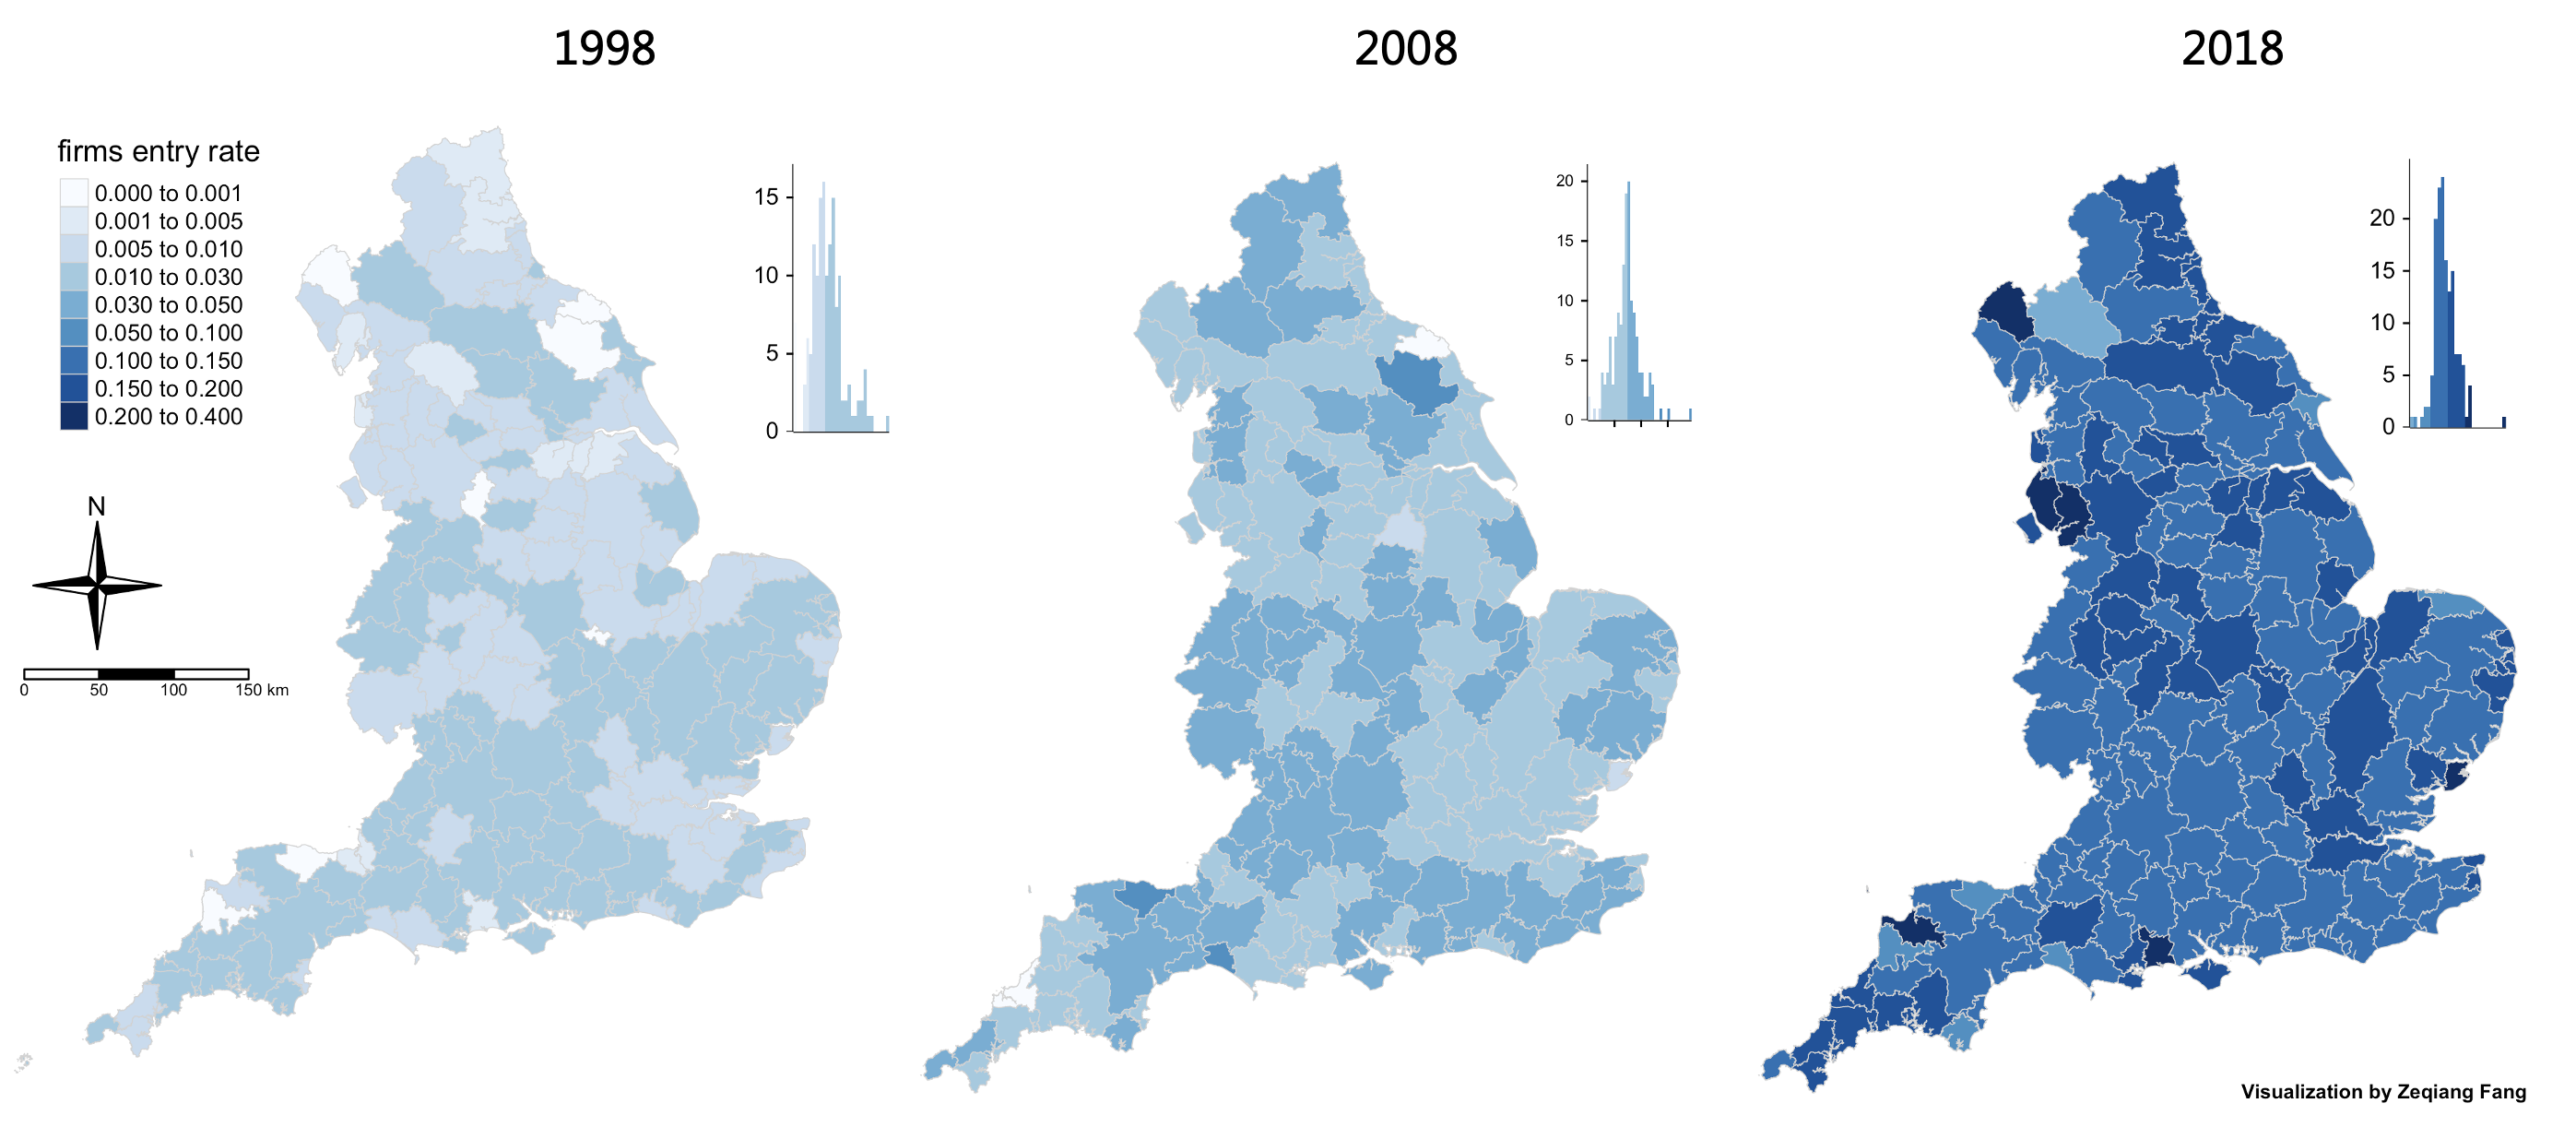
\includegraphics[width=1\linewidth]{/Users/fangzeqiang/Github/CASA0012-Dissertation/bookdown/general_images/enR_1998_2018} \caption{The distribution of the entry rate of the England tech clusters(ttwa) from 1998 to 2018}\label{fig:fig-enR-1998-2018}
\end{figure}

\hypertarget{descriptive-analysis}{%
\subsection{Descriptive Analysis}\label{descriptive-analysis}}

\hypertarget{visualisation-and-analysis-of-dynamics}{%
\section{Visualisation and Analysis of Dynamics}\label{visualisation-and-analysis-of-dynamics}}

\hypertarget{regression}{%
\subsection{Regression}\label{regression}}

For Top 10 clusters regression on the dynamics with year and location

\begin{figure}
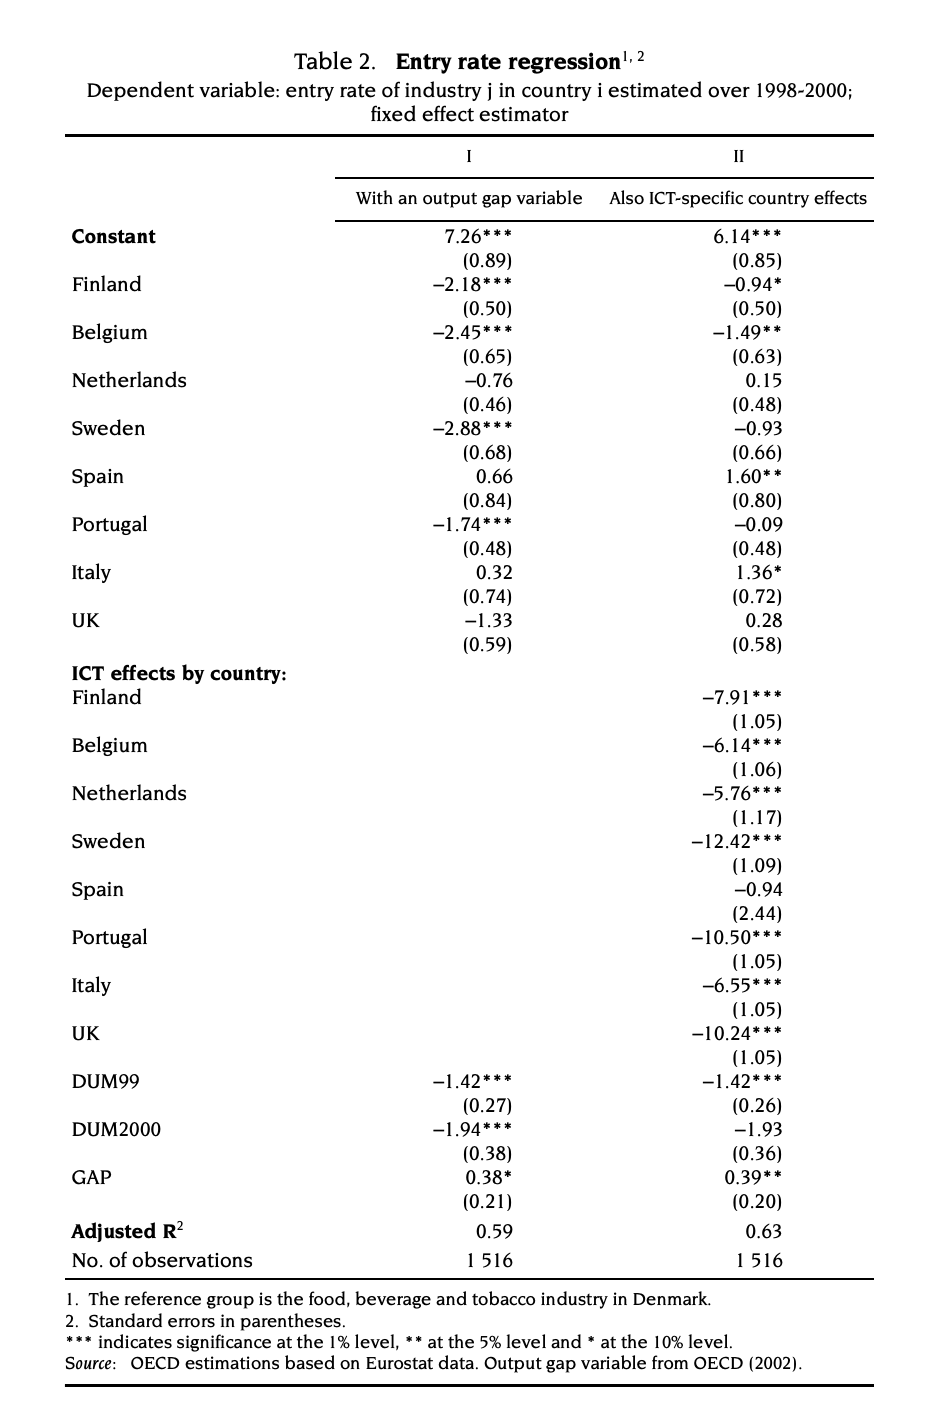
\includegraphics[width=1\linewidth]{/Users/fangzeqiang/Github/CASA0012-Dissertation/bookdown/general_images/entry_rate_regression} \caption{Regression results of tech clusters in England}\label{fig:fig-regression-entry-rate}
\end{figure}

xxx illustrates the unconditional relation between exit hazard rate and age. Consistent with \ldots, the exit hazard rate decreases with age. This is the case because on average entrants are less productive than incumbents. As a cohort ages -- see the right panel -- the survivors' productivity and value increase, leading to lower exit rates.

From \& Refer to \url{https://pages.stern.nyu.edu/~gclement/Papers/Entry_exit.pdf}

For Entry Rate \& HHI

\begin{figure}
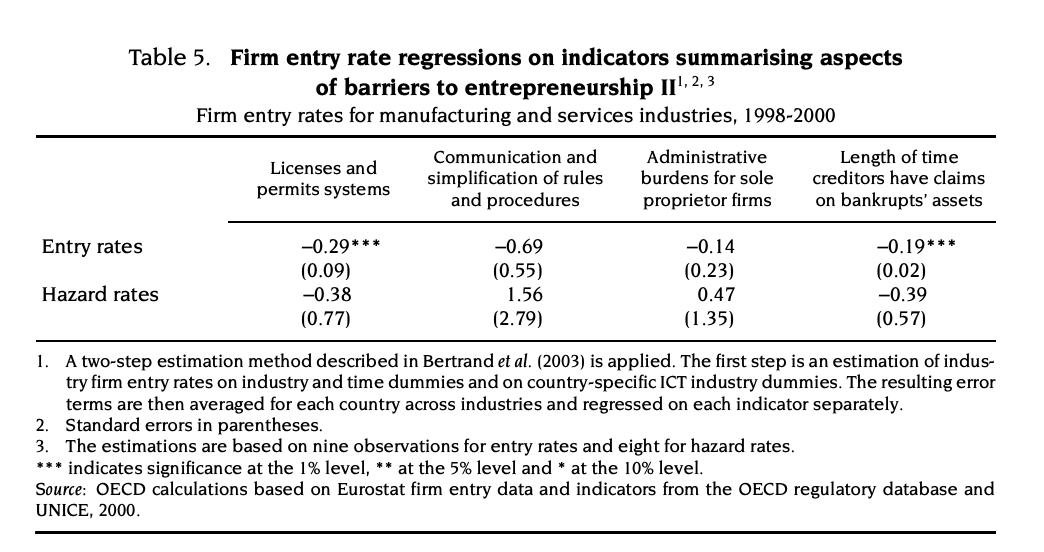
\includegraphics[width=1\linewidth]{/Users/fangzeqiang/Github/CASA0012-Dissertation/bookdown/general_images/two-dep-var-regression} \caption{Regression on industry mix and  dynamics of tech clusters in England}\label{fig:fig-regression-mix-entry}
\end{figure}

From \& Refer to \url{https://search.oecd.org/economy/growth/35027468.pdf}

\hypertarget{discussion}{%
\chapter{Discussion}\label{discussion}}

Short introduction to the chapter, reviewing the previous chapter and detailing what this one aims to achieve and build upon.

To be done

\hypertarget{research-significance}{%
\section{Research significance}\label{research-significance}}

\hypertarget{global-development-goals}{%
\subsection{Global development goals}\label{global-development-goals}}

\hypertarget{local-policy}{%
\subsection{Local policy}\label{local-policy}}

\hypertarget{academic-research}{%
\subsection{Academic research}\label{academic-research}}

\hypertarget{limitations-1}{%
\section{Limitations}\label{limitations-1}}

To be done

\hypertarget{transferability}{%
\section{Transferability}\label{transferability}}

To be done

\hypertarget{conclusion}{%
\chapter{Conclusion}\label{conclusion}}

case (Clementi \& Palazzo,2016)
This paper provides a framework to study the dynamics of the cross--section of firms and its implications for aggregate dynamics. When calibrated to match a set of moments of the investment process, our model delivers implications for firm dynamics and for the cyclicality of entry and exit that are consistent with the evidence.

The survival rate increases with size. The growth rate of employment is decreasing with size and age, both unconditionally and conditionally. The size distribution of firms is skewed to the right. When tracking the size distribution over the life a cohort, the skewness declines with age. The entry rate is positively correlated with current and lagged output growth. The exit rate is negatively correlated with output growth and positively associated with future growth.

Carefully modeling firm--level dynamics turns out to be key. The pro--cyclicality of entry and the positive association between age and firm growth deliver amplification and propagation of aggregate shocks in a plain-vanilla competitive framework.

A positive shock to aggregate productivity leads to an increase in entry. Consistent with the empirical evidence, entrants are smaller than incumbents. The skewness of the distribution of firms over idiosyncratic productivity increases. As the exogenous component of aggregate productivity declines towards its unconditional mean, the new entrants that survive grow in productivity and size. That is, the distribution of idiosyncratic productivity improves. As a result, the response of output is stronger and more persistent than in an environment that abstracts from entry and exit.

Our numerical experiments reveal that on average, entry and exit account for about one fifth of the above--trend growth experienced by our economy over the 10 years following a 1.5 standard deviation innovation to aggregate productivity. As an alternative metric of the impact of entry and exit on aggregate dynamics, we assessed the effect on persistence. For a version of our model without entry or exit to generate a data--conforming persistence of output, the first--order autocorrelation of aggregate productivity shocks must be 0.775. In the benchmark scenario with entry and exit, it needs only be 0.685.

Last, but not least, we show that according to our model there is a clear causal link between the exceptionally large drop in establishments during the great recession and the painfully low speed of the recovery from it. Whatever its exact nature, the adverse event that initiated the recession had a particularly strong effect on the 2008 and 2009 cohorts, severely reducing the ranks of small but high--conditional--growth plants and thereby suppressing the growth in aggregate labor demand for years to come.

In spite of the wealth of detail and descriptive realism achieved by the model, our framework could be extended in a variety of dimensions. In particular, we would like to gauge the quantitative effect of our mechanism when imbedded in a genuine general equilibrium framework. Relaxing our assumption that firms of different cohorts share the same technology is also of interest. Assuming, as it appears to be the case in reality, that entrants are more likely to adopt more recent vintages of capital, is likely to further enhance the amplification and propagation mechanism uncovered here.
end (Clementi \& Palazzo,2016)

\hypertarget{references}{%
\chapter*{References}\label{references}}
\addcontentsline{toc}{chapter}{References}

a b c d e f g h i j k l m n o p q r s t u v w x y z
pay attention to the unity of format

ALCACER J. and CHUNG W. (2007) Location strategies and knowledge spillovers, Management Science 53, 760--776.

Brandt, N., 2005. Business dynamics and policies. OECD Economic Studies, 2004(1), pp.9-36.

Burgess, G., Monk, S., Morrison, N. and Udagawa, C., 2014. Economic Analysis of the Wisbech Travel to Work Area: Main Report: March 2014.

Baptista, R. and Swann, G., 1999. A comparison of clustering dynamics in the US and UK computer industries. Journal of Evolutionary Economics, 9(3), pp.373-399.

Boschma, R., 2015. Do spinoff dynamics or agglomeration externalities drive industry clustering? A reappraisal of Steven Klepper's work. Industrial and Corporate Change, 24(4), pp.859-873.

Combes, P.-P., Duranton, G., Gobillon, L., Puga, D. and Roux, S. (2012),The Productivity Advantages of Large Cities: Distinguishing AgglomerationFrom Firm Selection. Econometrica, 80: 2543-2594.https://doi.org/10.3982/ECTA84427

Clementi, G.L. and Palazzo, B., 2016. Entry, exit, firm dynamics, and aggregate fluctuations. American Economic Journal: Macroeconomics, 8(3), pp.1-41.

Frenken, K., Cefis, E., \& Stam, E. 2015. Industrial Dynamicsand Clusters: A Survey. Regional Studies, 49(1), 10-27.doi:10.1080/00343404.2014.904505

Hall, B.L., Hsiao, E.Y., Majercik, S., Hirbe, M. and Hamilton, B.H., 2009. The impact of surgeon specialization on patient mortality: examination of a continuous Herfindahl-Hirschman index. Annals of surgery, 249(5), pp.708-716.

Kerr, William R., and Frederic Robert-Nicoud. 2020. ``Tech Clusters.''Journal of Economic Perspectives, 34 (3): 50-76.https://www.aeaweb.org/articles?id=10.1257/jep.34.3.50

Kwoka, J., 1977. Large Firm Dominance and Price-Cost Margins in Manufacturing Industries. Southern Economic Journal, 44(1), p.183.

Krafft, J., 2004. Entry, exit and knowledge: evidence from a cluster in the info-communications industry. Research policy, 33(10), pp.1687-1706.

Liston-Heyes, C. and Pilkington, A., 2004. Inventive concentration in the production of green technology: A comparative analysis of fuel cell patents. Science and Public Policy, 31(1), pp.15-25

Lu, C., Qiao, J. and Chang, J., 2017. Herfindahl--Hirschman Index based performance analysis on the convergence development. Cluster Computing, 20(1), pp.121-129.

Mateos-Garcia, J. and Bakhshi, H., 2016. The geography of creativity in the UK. London: Nesta.

Open Corporates. 2018, The core company data from OpenCorporates master company database, electronic dataset, OpenCorporates Data Dictionary, viewed 12 June 2021, \url{https://opencorporates.com/}.

Office for National Statistics, 2015. Identifying Science and Technology Businesses in Official Statistics. {[}online{]} London, UK: Office for National Statistics, pp.10-14. Available at: \url{https://webarchive.nationalarchives.gov.uk/20160105170025/http://www.ons.gov.uk/ons/site-information/using-the-website/rss-news-feeds/index.html} {[}Accessed 28 July 2021{]}.

Prothero, R., 2021. Travel to work area analysis in Great Britain. {[}online{]} Office for National Statistics. Available at: \url{https://www.ons.gov.uk/employmentandlabourmarket/peopleinwork/employmentandemployeetypes/articles/traveltoworkareaanalysisingreatbritain/2016} {[}Accessed 8 August 2021{]}.

Titheridge, H. and Hall, P., 2006. Changing travel to work patterns in South East England. Journal of Transport Geography, 14(1), pp.60-75.

\addcontentsline{toc}{chapter}{Bibliography}
\printbibliography

\hypertarget{appendix-a-classification-form}{%
\chapter*{Appendix A Classification Form}\label{appendix-a-classification-form}}
\addcontentsline{toc}{chapter}{Appendix A Classification Form}

\addtocontents{toc}{\protect\setcounter{tocdepth}{0}}

\hypertarget{science-and-technology-classification}{%
\section*{Science and Technology Classification}\label{science-and-technology-classification}}

\hypertarget{appendix-b-proposal}{%
\chapter*{Appendix B Proposal}\label{appendix-b-proposal}}

\addtocontents{toc}{\protect\setcounter{tocdepth}{3}}
\enddocument

\printbibliography

\end{document}
